\documentclass{article}
\usepackage{todonotes}
\usepackage{tikz}
\usetikzlibrary{arrows,automata}

\title{FraCaS: 80 percent complete}

% - Two-phase system (Dyn semantics from theorem proving)
% - Anaphora (as in Jolli paper) --- but this is the first time that this is done for FraCas.
% - Multiple readings
% - Threshold-based interpretation of (some) adjectives + Linear arithmetic proofs
% - New handling of prepositions and adverbs
% - Definites handled by adding an assumption at the top-level. (instead as inline existential) -- Enabled by dyn. semantics
% - Plurals/Quantifiers improved
% - Genders are properties of nouns
% - Handling of comparatives (with threshold BUT not those of adjectives), relying largely on the dyn. semantic system

\begin{document}



\section{Introduction}

\paragraph{Contributions}
(see list above)
\section{Background}

\section{Overview of the system}
% - Two-phase system (Dyn semantics from theorem proving)
% - Multiple readings

\begin{figure}
  \centering
{
  \tiny
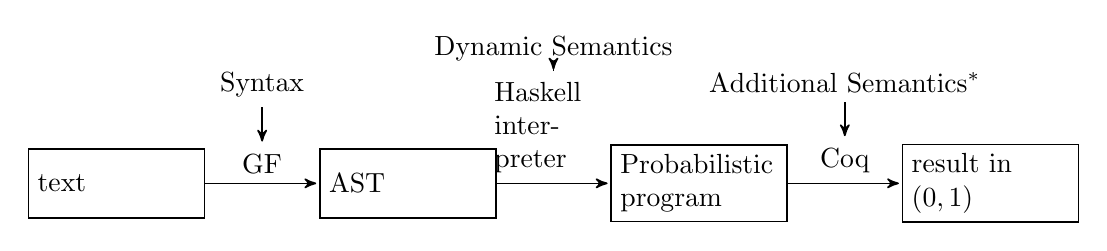
\begin{tikzpicture}[->,>=stealth',shorten >=1pt,auto,node distance=3.7cm,
                    semithick]
  \tikzstyle{every state}=[draw=black,text=black,shape=rectangle,text width=2cm]

  \node[state]         (txt)                {text};
  \node[state]         (ast) [right of=txt] {AST};
  \node[state]         (pp)  [right of=ast] {Probabilistic program};
  \node[state]         (res) [right of=pp] {result in $(0,1)$};

  \path (txt) edge              node (GF)  {GF}                  (ast)
        (ast) edge              node (Hask) [text width=1.5cm]{Haskell interpreter} (pp)
        (pp) edge               node (Coq) {Coq} (res);

  \node (Syntax) [above of=GF,node distance=1cm] {Syntax};
  \node (Sem) [above of=Hask,node distance=1cm] {Dynamic Semantics};
  \node (Hyper) [above of=Coq,node distance=1cm] {Additional Semantics$^\ast$};

  \path
  (Syntax) edge (GF)
  (Sem) edge (Hask)
  (Hyper) edge (Coq);
\end{tikzpicture}
}  
\caption{Phases in our system. ($\ast$) At the level of Coq, we handle
  the details of the adverbial (veridicality properties) and
  adjectival semantics (division into subsective, extentional,
  non-committal, etc. categories.) }
  \label{fig:overview}
\end{figure}

\subsection{Salient points}
% - Dynamic Semantics/Anaphora (as in Jolli paper) --- but this is the first time that this is done for FraCas.
%   -> Gender is a property of nouns
% - Definites handled by adding an assumption at the top-level. (instead as inline existential) -- Enabled by dyn. semantics
% - Handling of comparatives (with threshold BUT not those of adjectives), relying largely on the dyn. semantic system
% - Threshold-based interpretation of (some) adjectives + Linear arithmetic proofs (Automation)
% - New handling of prepositions and adverbs


\section{Results and evaluation}
% - show overall numbers
% - compare with others
% - error analysis (classify, show examples)

\section{Future work}
\section{Conclusion}




\end{document}